\section{The scaling-control problem as a benchmark}\label{sec:benchmark}

\subsection{Philippine industrial context}\label{sec:phcontext}

The Philippines operates among the world's largest installed geothermal
capacities, dominated by liquid-dominated fields whose separated brines
leave the flash plant at or near amorphous-silica
saturation~\citep{fronda2020country}. Polymerization of that silica
sets the effective floor on reinjection temperature, and with it the
ceiling on bottoming-cycle heat recovery, across fields of the Bacman
and Tiwi type whose chemistry anchors this work. The endmember brine
envelope is taken from the Tiwi geochemical
survey~\citep{sugiaman2004geochemical}; twenty years of geochemical
records at Bacman document how far a single field's chemistry can
wander over an operating life~\citep{espartinez2015bacman}.

Mitigation practice at these fields is documented and, importantly for
what follows, static. The record includes inhibitor hot-injection
trials at BacMan-II~\citep{see2010wgc}, field tests of pH
modification~\citep{remoroza2008ph}, a sustained phosphino-carboxylate
inhibitor program~\citep{baltazar2014grc}, and manual management of
reinjection lines~\citep{kobayashi2024mahanagdong}. These programs form
the empirical baseline against which our controller is benchmarked;
none of them closes a model-based loop. Economic quantities throughout
are peso-denominated, with every coefficient declared as a scenario
band. Where trade-press figures inform a scenario, notably the
400~kg/s Bacman-scale brine stream, they set scale only and are never
fitted to or used as validation targets; the repository enforces this
rule in code.

\subsection{Chemistry as control structure}\label{sec:chemistry}

Read in control language, silica scaling is a constraint process with
four features that together make it a demanding benchmark for economic
optimization under mismatch. The classical rate correlation is a
fourth-order peak-rate law in
supersaturation~\citep{rothbaum1979rohde}, so modest errors in
chemistry or temperature are raised to the fourth power exactly where
the constraint binds. The rate constant is non-Arrhenius above roughly
90~$^{\circ}$C: a low-temperature Arrhenius fit ($E_a = 9.1$~kJ/mol
over 5--90~$^{\circ}$C) overpredicts $k$ at 150~$^{\circ}$C by a factor
of 3.0 (Fig.~\ref{fig:arrhenius}), which means extrapolating cold-lab
kinetics to a hot brine line is quantitatively wrong rather than merely
imprecise. The process carries an induction delay, with onset lagging
supersaturation exposure and the induction period falling steeply in
supersaturation ($P \propto s^{-4.3}$, $r^2 = 0.88$, fitted from the
same primary dataset). Finally, the inhibitor actuator is
non-monotonic~\citep{gallup2002investigations}: the best organic
formulation suppressed deposition by more than half near 1~ppm, and
inhibition then decreased at higher dosage. Dosing is therefore a
genuine optimization problem, not a saturating knob.

Solubility sets the economic stakes of the temperature lever. Using the
primary amorphous-silica correlation of \citet{gunnarsson2000amorphous}
with the Tiwi archetype brine, cooling the reinjection line from 150 to
90~$^{\circ}$C raises the uninhibited polymerization rate by a factor
of about 101 (Fig.~\ref{fig:lever}). Every degree of additional heat
recovery is purchased at a steeply nonlinear scaling price, which is
why a static policyleaves either megawatts or safety margin on the
table.

\begin{figure}[t]\centering
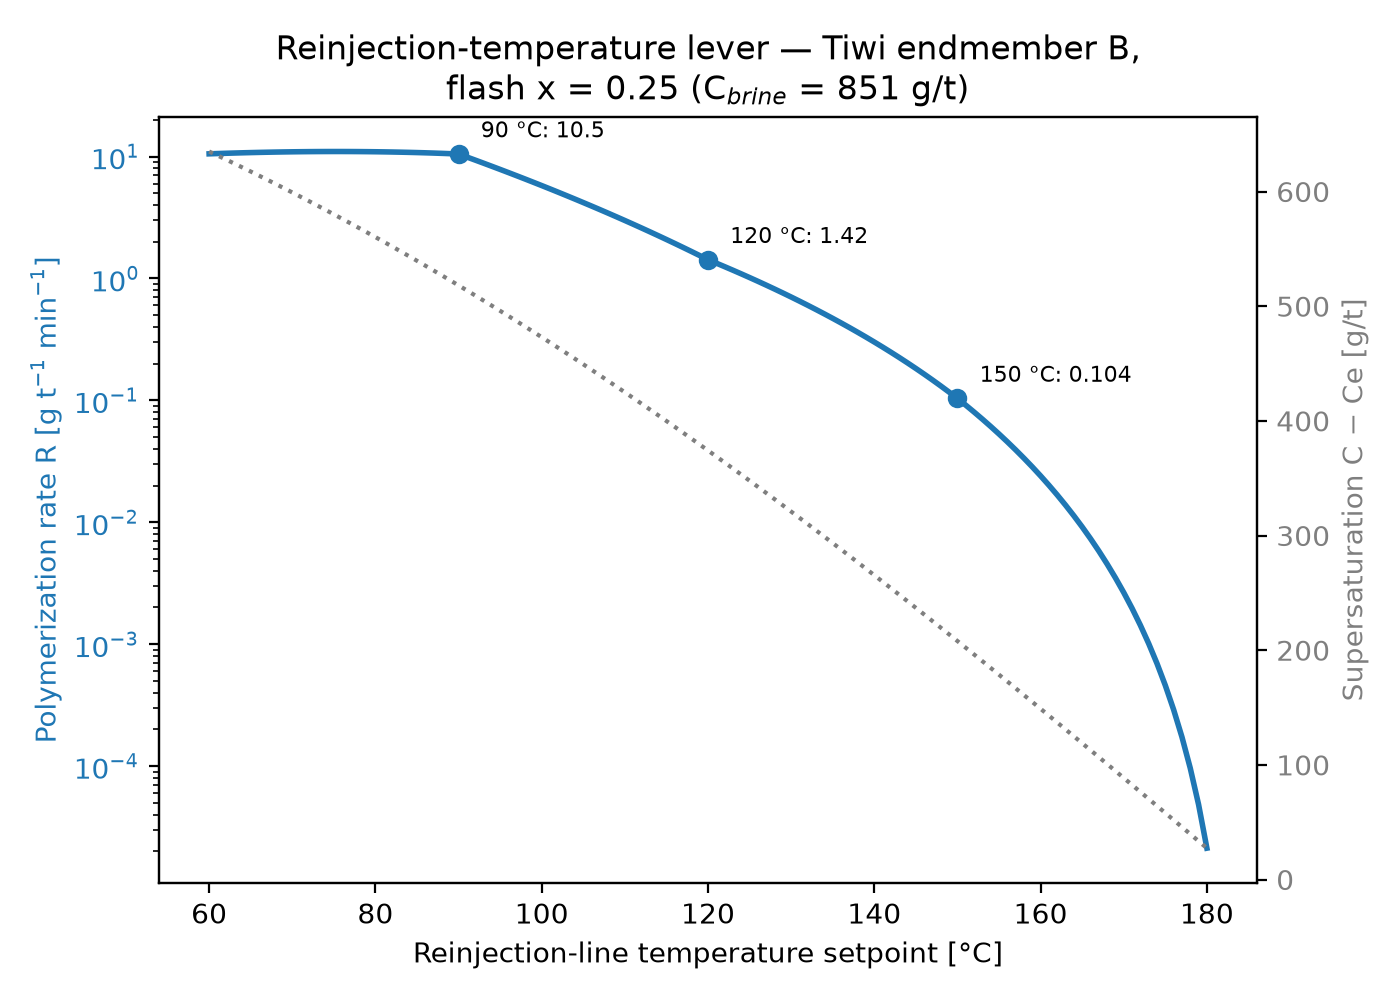
\includegraphics[width=.72\linewidth]{fig_temperature_lever.png}
\caption{The reinjection-temperature lever. Uninhibited polymerization
rate along the brine line versus temperature set-point for the
archetype brine (Tiwi endmember B, 638~mg/kg reservoir
silica~\citep{sugiaman2004geochemical}; flash fraction $x = 0.25$,
scenario input; solubility from \citet{gunnarsson2000amorphous};
kinetics from the checksum-validated transcription of
\citet{rothbaum1979rohde}). Cooling from 150 to 90~$^{\circ}$C raises
the rate by a factor of 101.}\label{fig:lever}
\end{figure}
\begin{figure}[t]\centering
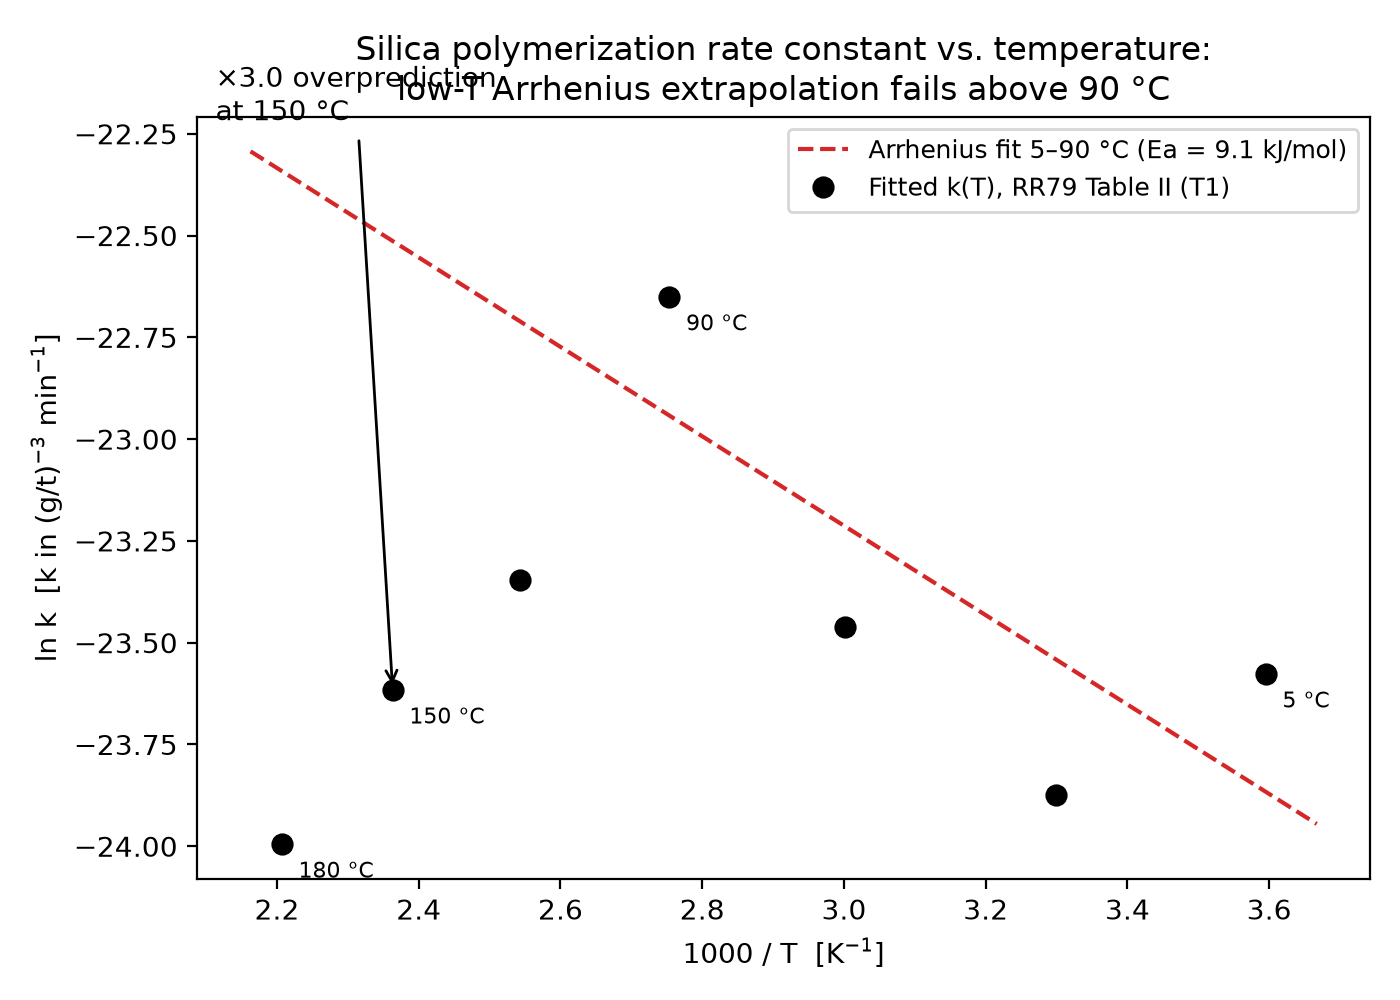
\includegraphics[width=.72\linewidth]{fig_arrhenius_overprediction.png}
\caption{Fitted fourth-order rate constants $k(T)$ over
5--180~$^{\circ}$C, regenerated from the primary transcription of
\citet{rothbaum1979rohde}. The dashed Arrhenius fit to the
5--90~$^{\circ}$C nodes ($E_a = 9.1$~kJ/mol) overpredicts $k$ at
150~$^{\circ}$C by a factor of 3.0.}\label{fig:arrhenius}
\end{figure}
